% ==========================================================================================
% ==========================================================================================
% ==========================================================================================

\def\myname{John Terhorst}
\def\myshortname{Terhorst, J.}
\def\mydoctitle{Document Title}
\def\myfontsize{11pt}
\def\mymargins{1.1in}

% ==========================================================================================
% ==========================================================================================
% ==========================================================================================

\documentclass[letterpaper,\myfontsize]{article}
%\documentclass[letterpaper,titlepage,\myfontsize]{article}
%\documentclass[letterpaper,twocolumn,\myfontsize]{article}
\usepackage[top=\mymargins, bottom=\mymargins, left=\mymargins, right=\mymargins]{geometry} % showframe

% ==========================================================================================
% ==========================================================================================
% ==========================================================================================

% basic setup - for font packages see http://www.tug.dk/FontCatalogue/

% \renewcommand{\familydefault}{\sfdefault}   % \rmdefault, \sfdefault, \ttdefault
% \usepackage[T1]{fontenc} % use for accented chars like \"o or \AA or \'e
% \usepackage[tracking=true,kerning=true,factor=1100,stretch=10,shrink=10]{microtype}
\usepackage{microtype,verbatim}
% \usepackage[version=4]{mhchem}  % use arrows=pgf-filled if using mathptmx or newtxtext/newtxmath
\usepackage{parskip}
% \usepackage{ulem}
% textcomp,siunitx,textgreek,float
% \usepackage[calligra]{emf} % alternate to mathrsfs \mathscr{E}
% \usepackage{tikz} % remove if no tikz
% \usepackage{mathptmx}   
% \usepackage{enumitem} % can use [noitemsep] in itemize 
% \usepackage{chemfig}\setchemfig{atom sep=2em}\setchemfig{angle increment=30} % see chemfig
% \usepackage[bottom,hang,symbol]{footmisc}\setlength\footnotemargin{9pt}\interfootnotelinepenalty=10000\setlength{\skip\footins}{0.5cm}  % if used, must go after setspace
% \usepackage{setspace}\setstretch{1.1} % if used, must go before geometry
\usepackage[all]{nowidow} % widow/orphan prevention

% ==========================================================================================
% ==========================================================================================
% ==========================================================================================

% natbib references

\usepackage[super,comma,sort&compress]{natbib}
\renewcommand{\bibnumfmt}[1]{#1.}
% \renewcommand{\refname}{References}
% \let\oldbibliography\thebibliography\renewcommand{\thebibliography}[1]{\oldbibliography{#1}\setlength{\itemsep}{3pt}}
\newcommand*\myaref[6]{\bibitem{#1}#2 \textit{#3} \textbf{#4}, \textit{#5}, #6.} 
\newcommand*\mytref[7]{\bibitem{#1}#2 ``#3.'' \textit{#4} \textbf{#5}, \textit{#6}, #7.} % with title
\newcommand*\myzref[8]{\bibitem{#1}#2 ``#3.'' \textit{#4} \textbf{#5}, \textit{#6}(#7), #8.} % with title and issue

% ==========================================================================================
% ==========================================================================================
% ==========================================================================================

% tables and figures

\usepackage{booktabs}
\setlength\heavyrulewidth{0.15ex}\setlength\cmidrulewidth{0.1ex}\setlength\lightrulewidth{0.1ex}

\usepackage{graphicx}
\usepackage[font=normalsize,labelfont={bf},margin=1in]{caption}\captionsetup[table]{aboveskip=3pt}\captionsetup[figure]{skip=3pt}
% \setlength{\textfloatsep}{9pt plus 1.0pt minus 2.0pt} % adjust space from caption to body text

% ==========================================================================================
% ==========================================================================================
% ==========================================================================================

% section headers - \bfseries, \rmseries, \itshape, \slshape (use instead of \it for sffamily), \scshape

\usepackage{titlesec} 
% \usepackage[explicit]{titlesec} % use [explicit] to include arg #1 as in example for underline
% \titleformat{\section}[block]{\filcenter}{\thetitle.}{0.5em}{\textsc{#1}} % centered title - very nice as \section*
% \titleformat{\section}{\bbb\bfseries}{\thetitle.}{.5em}{}
\titleformat{\section}{\large\bfseries}{\thetitle.}{.5em}{}
\titleformat{\subsection}{\large\bfseries}{\thetitle.}{.5em}{}
% \titleformat{\subsection}{\normalsize\itshape}{\thetitle.}{.5em}{}
% \titleformat{\subsection}{\normalfont}{\thesubsection.}{.5em}{\uline{#1}} % requires ulem
% \titleformat{\subsection}{\itshape}{\thesubsection.}{.5em}{\uline{#1}}
% \titleformat{\subsubsection*}{\itshape}{\thesubsubsection*.}{.5em}{}
% \makeatletter\def\@seccntformat#1{\llap{\csname the#1\endcsname\quad}}\makeatother %this puts header numbers in margin

%                       indent    vskip before               vskip after
% \titlespacing\section{0pt}{13pt plus 0pt minus 0pt}{11pt plus 0pt minus 0pt}
% \titlespacing\subsection{0pt}{13pt plus 0pt minus 0pt}{11pt plus 0pt minus 0pt}
% \titlespacing\paragraph{0pt}{13pt plus 0pt minus 0pt}{5pt plus 2pt minus 2pt}

% ==========================================================================================
% ==========================================================================================
% ==========================================================================================

% TOC stuff

% \usepackage{titletoc} - provides additional toc features

% ==========================================================================================
% ==========================================================================================
% ==========================================================================================

% environments

% \usepackage{enumerate}

% \newenvironment{qnumerate}
% {\begin{enumerate}[\bf{Q}1.]}{\end{enumerate}}

% \newenvironment{anumerate}
% {\begin{enumerate}[\bf(a)]}{\end{enumerate}}

% ==========================================================================================
% ==========================================================================================
% ==========================================================================================

% fancy page headers

% built-in function
% \pagestyle{myheadings}
% \markboth{left}{\textnormal{\myshortname} \textit{\mydoctitle}}

% \usepackage{lastpage}
% \usepackage{fancyhdr} 
% \renewcommand{\headrulewidth}{0pt} % this is the header hrule line
% \setlength{\headsep}{0.2in}
% \setlength{\headheight}{13.7pt}

% \usepackage{fancyhdr} 
%        \lhead{} 
%        \chead{} 
%        \rhead{\textit{\mydoctitle}} 
%        \lfoot{} 
%        \cfoot{\thepage}
%        \rfoot{} 
%        \setlength{\headheight}{14.5pt}
%        \pagestyle{fancy} % empty, plain, fancy - use \thispagestyle{fancy} for indiv pages

% \fancypagestyle{custom}
%  {
%   \fancyhead[L]{}
%   \fancyhead[R]{}
%   \fancyfoot[C]{Page \thepage\ of \pageref{LastPage}}
%   \fancyfoot[C]{\thepage}
%  } 
% \pagestyle{custom}

% ==========================================================================================
% ==========================================================================================
% ==========================================================================================

% macros

% \newcommand*\supr[1]{$^{#1}$}
% \newcommand*\sub[1]{$_{#1}$}
% \newcommand*\unit[1]{\textnormal{ #1}}
% \newcommand*\rsq[1]{Correlation coefficient for line of best fit is $R^2=#1$}

% ==========================================================================================
% ==========================================================================================
% ==========================================================================================

% labels

% \def\tablab{Table}\def\tabslab{\tablab s}
% \def\figlab{Figure}\def\figslab{\figlab s}
% \def\equlab{Eq.}\def\equslab{Eqs.}
% \newcommand*\eq[1]{\equlab~\ref{#1}}
% \newcommand*\eqs[1]{\equslab~\ref{#1}}
% \newcommand*\tbl[1]{\tablab~\ref{#1}}
% \newcommand*\fig[1]{\figlab~\ref{#1}}
% \newcommand*\figs[1]{\figslab~\ref{#1}}

% ==========================================================================================
% ==========================================================================================
% ==========================================================================================

% shortcuts

% \def\deg{$^{\circ}$}
% \def\degc{$^{\circ}$C}
% \def\dcrt{25 $^{\circ}$C}
% \def\tild{$\sim$}
% \def\delg{$\Delta G$}
% \def\dgnot{$\Delta G^\circ$}
% \def\dgfnot{$\Delta G_\textnormal{f}^\circ$}
% \def\dgrxn{$\Delta G_\textnormal{rxn}$}
% \def\dgnotrxn{$\Delta G_\textnormal{rxn}^\circ$}
% \def\delh{$\Delta H$}
% \def\dhrxn{$\Delta H_\textnormal{rxn}$}
% \def\dhnotrxn{$\Delta H_\textnormal{rxn}^\circ$}
% \def\dhnot{$\Delta H^\circ$}
% \def\dhf{$\Delta H_\textnormal{f}$}
% \def\dhfnot{$\Delta H_\textnormal{f}^\circ$}
% \def\dhfus{$\Delta H_\textnormal{fus}$}
% \def\dhvap{$\Delta H_\textnormal{vap}$}
% \def\dhfnot{$\Delta H_\textnormal{f}^\circ$}
% \def\dsnotrxn{$\Delta S_\textnormal{rxn}^\circ$}
% \def\dsnot{$\Delta S^\circ$}
% \def\dels{$\Delta S$}
% \def\essnot{$S^\circ$}
% \def\electron{e$^-$}
% \def\Ecell{$\emf_{\hspace*{-.3mm}\textnormal{cell}}$}
% \def\Enotcell{$\emf^{\hspace*{.5mm}\circ}_{\hspace*{-.3mm}\textnormal{cell}}$}
% \def\Enot{$\emf^{\hspace*{.5mm}\circ}$}
% \def\Ka{$K_{\textnormal{a}}$}
% \def\Kb{$K_{\textnormal{b}}$}
% \def\Ksp{$K_{\textnormal{sp}}$}
% \def\Keq{$K_{\textnormal{eq}}$}
% \def\Kp{$K_P$}
% \def\Kc{$K_{\textnormal{c}}$}
% \def\pKa{p$K_{\textnormal{a}}$}
% \def\pKb{p$K_{\textnormal{b}}$}
% \def\haber{\ce{N2(g) + 3H2(g) -> 2NH3(g)}}
% \def\dipole{+\hspace*{-3mm}$\longrightarrow$}
% \def\cmi{cm$^{-1}$}
% \def\cd{$\cdot$}
% \def\dd{\end{document}} % useful for debugging
% \newcommand*\ph[1]{$\textnormal{pH}=#1$}
% \newcommand*\Kan[2]{$K_{\textnormal{a}_{#1}}=\num{#2}$}

% fractions

% \usepackage{nicefrac}
% \def\half{\nicefrac{1}{2}}
% \def\third{\nicefrac{1}{3}}
% \def\quarter{\nicefrac{1}{4}}
% \def\threequarter{\nicefrac{3}{4}}
% \def\twothird{\nicefrac{2}{3}}


% ==========================================================================================
% ==========================================================================================
% ==========================================================================================

% hyperref, load last

% \PassOptionsToPackage{hyphens}{url} % hyperref uses url package; this enables extra hyphenation for long urls
% \usepackage[pdftex]{hyperref}
% \urlstyle{same} % use roman instead of typewriter for url
% \hypersetup{ colorlinks = true,
%              linkcolor = true, 
%              urlcolor = black,
%              pdfauthor = {\myname},
%              pdfkeywords = {\mydoctitle},
%              pdftitle = {\mydoctitle},
%              pdfsubject = {\mydoctitle},
%              pdfpagemode = UseThumbs }

% ==========================================================================================
% ==========================================================================================
% ==========================================================================================

% maketitle definitions

\title{\vspace*{-1.51cm}\mydoctitle}
%\author{\normalsize\myname}
\date{\today}

\usepackage{authblk}
\author[1,2]{\myname}
\author[2]{Erin Schwartz}
\author[2]{Heather Glasser}
\affil[1]{Division of Natural Sciences, Vanguard University, Costa Mesa, CA 92626}
\affil[2]{Department of Chemistry, University of Redlands, Redlands, CA, 92373}

\begin{document}%\maketitle


% ==========================================================================================
% ==========================================================================================
% ==========================================================================================

% front matter
%\pagestyle{empty}
\maketitle
\begin{comment}
\tableofcontents
\newpage
\pagestyle{plain}
\setcounter{page}{1}
\pagenumbering{roman}
\addcontentsline{toc}{section}{List of Figures}
\listoffigures
\newpage
\addcontentsline{toc}{section}{List of Tables}
\listoftables
\newpage
\setcounter{page}{1}
\pagenumbering{arabic}
\end{comment}

% ==========================================================================================
% ==========================================================================================
% ==========================================================================================

\section{Introduction}

Health goth~\cite{heitlon,ez} letterpress portland chicharrones cornhole ethical. Coloring book dreamcatcher ethical single-origin coffee listicle, tacos venmo enamel pin retro bushwick. Polaroid deep vee umami, locavore subway tile adaptogen crucifix kickstarter pour-over waistcoat cliche selvage. Migas echo park next level salvia art party. Kinfolk etsy you probably haven't heard of them kickstarter narwhal, fingerstache schlitz disrupt meggings three wolf moon twee waistcoat actually austin organic. Yr hot chicken cardigan, fanny pack leggings tbh next level cornhole.

\smallskip
\begin{figure}[htbp]
\centering
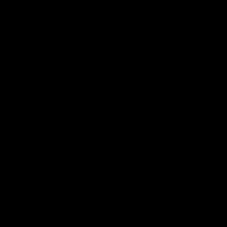
\includegraphics[scale=0.25]{square.jpg}
\caption{The pairwise nature of the Born radius.}
\label{bornrad}
\end{figure}%

Lorem ipsum dolor sit amet, consectetur adipiscing elit, sed do eiusmod tempor incididunt ut labore et dolore magna aliqua. Feugiat vivamus at augue eget arcu. Donec et odio pellentesque diam volutpat commodo sed egestas egestas. Sem nulla pharetra diam sit amet. Sagittis purus sit amet volutpat consequat mauris. Urna cursus eget nunc scelerisque viverra mauris in aliquam. Nec dui nunc mattis enim. Rhoncus aenean vel elit scelerisque mauris pellentesque pulvinar. Cras fermentum odio eu feugiat pretium nibh ipsum. Luctus accumsan tortor posuere ac ut consequat semper. Suscipit tellus mauris a diam maecenas sed enim ut. Posuere lorem ipsum dolor sit amet consectetur adipiscing. 

Duis tristique sollicitudin nibh sit amet commodo nulla. Bibendum est ultricies integer quis. Purus ut faucibus pulvinar elementum integer enim. Pretium lectus quam id leo in vitae turpis massa. Vulputate enim nulla aliquet porttitor lacus luctus accumsan. Sapien et ligula ullamcorper malesuada proin libero nunc consequat. Tortor id aliquet lectus proin nibh nisl condimentum id. Nibh tortor id aliquet lectus proin nibh nisl.

\begin{table}[htbp]
\centering
\caption{Gravimetric analysis of silver halides in a 1.27-mL sample of Salton Sea water.}
\begin{tabular}{cc}
\toprule
A & B \\
\midrule
C & D \\
\bottomrule      
\end{tabular}
\label{tabgrav}
\end{table}

Tellus in hac habitasse platea. Lectus quam id leo in vitae turpis massa sed. A condimentum vitae sapien pellentesque habitant morbi tristique. Velit sed ullamcorper morbi tincidunt. Volutpat est velit egestas dui id ornare arcu. Ipsum dolor sit amet consectetur adipiscing elit duis tristique. Tellus orci ac auctor augue mauris augue neque. 

Vestibulum morbi blandit cursus risus at. Ornare lectus sit amet est placerat. Quam viverra orci sagittis eu volutpat odio facilisis mauris. Posuere ac ut consequat semper viverra nam libero justo laoreet. Phasellus egestas tellus rutrum tellus pellentesque eu tincidunt. Interdum varius sit amet mattis. Massa sapien faucibus et molestie ac feugiat sed lectus. Tellus cras adipiscing enim eu. Non diam phasellus vestibulum lorem.

% ==========================================================================================
% ==========================================================================================
% ==========================================================================================

\subsection{Procedure}

Eget aliquet nibh praesent tristique magna sit amet purus gravida. Sed viverra tellus in hac. Aliquet porttitor lacus luctus accumsan tortor posuere ac ut. Neque laoreet suspendisse interdum consectetur libero id. Amet risus nullam eget felis eget nunc lobortis mattis. Etiam sit amet nisl purus. Sit amet consectetur adipiscing elit ut aliquam purus. Eu lobortis elementum nibh tellus molestie nunc non. Egestas tellus rutrum tellus pellentesque eu tincidunt tortor aliquam nulla. Vitae suscipit tellus mauris a diam. Ut pharetra sit amet aliquam id diam maecenas ultricies mi. Suspendisse faucibus interdum posuere lorem.

% ==========================================================================================
% ==========================================================================================
% ==========================================================================================

\subsection{Materials}

Amet mauris commodo quis imperdiet. Facilisi nullam vehicula ipsum a arcu cursus. Sit amet dictum sit amet justo donec enim. Ac turpis egestas integer eget aliquet nibh. A arcu cursus vitae congue mauris. Augue lacus viverra vitae congue eu consequat ac. Congue quisque egestas diam in arcu cursus euismod quis. Tempus quam pellentesque nec nam. Pellentesque habitant morbi tristique senectus et netus et malesuada fames. Venenatis tellus in metus vulputate eu. Maecenas sed enim ut sem viverra aliquet eget. Quam lacus suspendisse faucibus interdum posuere lorem. Gravida dictum fusce ut placerat orci nulla. Tristique sollicitudin nibh sit amet commodo nulla facilisi nullam vehicula. Pretium lectus quam id leo in vitae turpis massa.











% ==========================================================================================
% ==========================================================================================
% ==========================================================================================

\newpage
\addcontentsline{toc}{section}{References}
\bibliographystyle{plain}
\begin{thebibliography}{200}
\mytref{heitlon}{Heitler, W.; London, F.}{Wechselwirkung neutraler Atome und hom\"oopolare Bindung nach der Quantenmechanik}{Phys.\ Lett.}{1927}{44}{455--473}
\myzref{ez}{Terhorst, J.\ P.; Jorgensen, W.\ L.}{\textsl{E/Z} Energetics for Molecular Modeling and Design}{J.\ Chem.\ Theory Comput.}{2010}{6}{9}{2762--2769}
\end{thebibliography}

% ==========================================================================================
% ==========================================================================================
% ==========================================================================================

\end{document}















% ==========================================================================================
% ==========================================================================================
% ==========================================================================================


% ==========================================================================================
% ==========================================================================================
% ==========================================================================================

% notes

%          with symbol, use \footnote[2]{text}
%          instead of 2 you can put the number of the symbol you like:
%          1   asterisk *   
%          2   dagger  
%          3   double dagger  
%          4   section symbol §   
%          5   paragraph ¶   
%          6   parallel lines  
%          7   two asterisks 
%          8   two daggers 
%          9   two double daggers 

% some fancy chem notation examples

\begin{center}
\ce{
Zn^2+
<=>[+ 2OH-][+ 2H+]
$\underset{\text{amphoteres Hydroxid}}{\ce{Zn(OH)2 v}}$
<=>[+ 2OH-][+ 2H+]
$\underset{\text{Hydroxozikat}}{\ce{[Zn(OH)4]^2-}}$
+ H2 ^
}
\end{center}    

% align environment

\begin{align*}
\ce{ A + B &->[+e] C \\
C &->[+e] D + E }
\end{align*}

